
\def \Subject {سیگنال تصویر و اضافه کردن نویز}
\def \Author {فرزان رحمانی}
\def \Session {1}
\setcounter{chapter}{\Session-1}

\chapter[\Subject]{\Subject}
% \BlankLine
\section{گام اول}
از قبل برنامه متلب را در کامپیوتر خود نصب داشتم و با آن کار کرده بودم. چرا که در ترم سوم برای درس مدار الکتریکی به آن نیاز داشتم.
\section{گام دوم}
در این گام عکسی را به عنوان ورودی برنامه‌مان انتخاب می‌کنیم.
\begin{figure}[H]
    \centering
    
\includegraphics[width=0.65\linewidth]{images/farzan.jpg}
    \caption{عکس ورودی}
    \label{fig:h}
\end{figure}
\subsection{بررسی کد}
حال کد متلب این گام را بررسی می‌کنیم
:

% \lr{\lstinputlisting{MatlabCode/step1.m}}
\lr{\lstinputlisting{MatlabCode/step2.m}}

حال به بررسی خطوط کد می‌پردازیم:
\begin{itemize}
    \item اول مسیر فایل داده‌شده را مشخص میکنیم
    \item سپس با دستور 
    \(imread\)
     آن فایل را می‌خوانیم
    \item
    و با دستور
    \(imshow\)
    فایل مرحله قبل را در خروجی نشان می‌دهیم.
\end{itemize}

\section{گام سوم}
در این گام با توجه به راهنمایی گفته شده در داک پروژه از تابع پیش تعریف‌شده 
\grayBox{
\(rgb2gray\)
}
استفاده می‌کنیم.
\\
\\
\subsection{بررسی کد}
حال کد متلب این گام را بررسی می‌کنیم
:
\lr{\lstinputlisting{MatlabCode/step3.m}}

\subsection{انواع تصاویر}
\begin{itemize}
    \item 
    \grayBox{binary images }
    : 
    این نوع تصاویر در یک ماتریس 
    \(m * n\)
    ذخیره می‌شوند که رنگ سیاه در آن معادل صفر و رنگ سفید معادل یک می‌باشد
    \item  
    \grayBox{indexed images  }
    :
    تصاویر نمایه‌ای یک نوع فرمت تصویر است که برای ذخیره‌ی تصاویر با پالت رنگی محدود استفاده می‌شود. در این نوع تصاویر، رنگ هر پیکسل به عنوان یک شاخص به جای مقدار رنگ RGB ذخیره می‌شود. با استفاده از یک جدول نمایه ، هر شاخص به مقدار واقعی رنگ تصویر تبدیل می‌شود.

به عبارت دیگر، تصاویر نمایه‌ای شامل مجموعه‌ای از شاخص‌ها هستند که به رنگ‌های مختلف متناظر هستند. این شاخص‌ها معمولاً عدد صحیح بین 0 و 255 هستند، که هر عدد نمایانگر یک رنگ است. از این روش برای کاهش حجم فایل تصویر و افزایش سرعت پردازش در برنامه‌ها استفاده می‌شود، زیرا نیاز به ذخیره‌سازی مستقیم مقادیر RGB برای هر پیکسل وجود ندارد.

به عنوان مثال، فرمت GIF یکی از نمونه‌های تصاویر نمایه‌ای است که می‌تواند تا 256 رنگ را در هر تصویر ذخیره کند. اما توجه داشته باشید که در تصاویر نمایه‌ای، تعداد رنگ‌ها محدود است و ممکن است منجر به کاهش کیفیت و دقت رنگ در تصویر شود.
    \item
    \grayBox{grayscale images }
     : 
    در
    این نوع تصاویر
    که در یک ماتریس
        \(m * n\)
ذخیره می‌شوند
    هر عضو آن شدت رنگ آن پیکسل را نشان می‌دهد.
   که بزرگترین عدد برای رنگ سفید و کوچکترین عدد برای رنگ سیاه می‌باشد 
   که با توجه به تایپ داده ها می‌توانند رنج مختلفی برای خود بگیرند 
   \begin{itemize}
       \item \lr{single or double} : \lr{[0,1]}
       \item \lr{uint8} : \lr{[0,..,255]}
        \item \lr{uint16} : \lr{ [0,...,65535]}
        \item int : \lr{[-32768,...,32768]}
   \end{itemize}
   \item \grayBox{truecolor images(rgb images)}
   : 
   این نوع تصاویر در یک ماتریس سه بعدی یعنی 
       \(m * n * 3\)
       ذخیره می شوند که به جای ذخیره کردن عدد در مرحله قبل یک ماتریس ۳ عضوی 
       متشکل از شدت رنگ های
       rgb
       (قرمز، آبی و سبز)
       را در خود نگه می دارد.

\end{itemize}
\section{گام چهارم}
تصویر تبدیل‌شده در مرحله قبل را با استفاده از تابع
imshow
نشان داده و آن را با استفاده از تابع
imwrite
ذخیره می‌کنیم.
\subsection{بررسی کد}
\lr{\lstinputlisting{MatlabCode/step4.m}}
\begin{figure}[H]
    \centering
    
\includegraphics[width=0.65\linewidth]{images/GrayImage.jpg}
    \caption{تصویر خاکستری‌شده  }
    \label{fig:h}
\end{figure}

\subsection{تفاوت فرمت های متفاوت عکس}
\begin{itemize}
    \item \grayBox{jpg}
    :
    این نوع تصاویر از نوع 
    فشرده‌سازی با اتلاف
    \footnote{compression lossy }
    می‌باشند.
    در 
    واقع حجم فایل را تا حد زیادی کاهش می‌دهد
    این نوع داده برای نگه‌داری و فرستادن مناسب است.
    این فرمت فایل از فشرده سازی با اتلاف برای تصاویر دیجیتال شما پشتیبانی می کند. این بدان معنی است که حجم فایل شما کاهش می یابد (فشرده سازی بیشتر مربوط به اندازه فایل های کوچکتر است). می توانید تصاویر را به میزان قابل توجهی کوچکتر کنید. قربانی این امر این است که کیفیت تصاویر شما کاهش می یابد (کمتر واضح هستند) زیرا فشرده سازی برخی از داده های اصلی را دور می اندازد تا تصویر کوچکتر شود. این به ویژه هر چه کوچکتر بروید صادق است.
    \item \grayBox{png}
    :
    این نوع تصایر از نوع فشرده‌سازی 
    بدون اتلاف
    \footnote{ compression lossless}
    می‌باشند.
    در واقع این نوع فشرده‌سازی مخالف فشرده‌سازی قبلی می‌باشد و می‌توان به بازسازی دوباره داده اصلی از فایل فشرده رسید.
    یک تصویر PNG برعکس فشرده سازی با اتلاف JPG است. از فشرده سازی بدون اتلاف پشتیبانی می کند. همانطور که از نام آن پیداست، "lessless" به توانایی آن در نگه داشتن تمام داده های اصلی در قالب فایل اشاره دارد. در نتیجه، کیفیت تصویر اصلی شما تغییر نمی کند یا کاهش نمی یابد. با این حال، معاوضه برای این مزیت این است که اندازه فایل بزرگتر از JPG خواهد بود. این می تواند در مورد سرعت وب سایت و UX برای بازدیدکنندگان وب سایت شما مشکل ساز باشد، زیرا تصاویر بزرگتر باعث می شود کل وب سایت زمان بیشتری برای بارگذاری طول بکشد.
    \item \grayBox{bmp}
    :
    توسط شرکت 
    Microsoft   
    توسعه یافته‌شده است.
    حجم فایل بیشتری دارد
    و از نوع 
    فشرده‌سازی بدون اتلاف می‌باشد.
    فرمت فایل بیت مپ یک فرمت جالب است زیرا استانداردی است که توسط مایکروسافت توسعه یافته و کلاسیک در نظر گرفته شده است. این بدان معنی است که به طور کلی در رابط های کاربری گرافیکی قدیمی استفاده می شود. طبیعتاً این یک فایل تصویری بزرگتر است. با این حال، می‌توانید آن را با فناوری ZIP تحت فشرده‌سازی بدون تلفات قرار دهید.
    \item \grayBox{tiff}
    :
    این نوع نسبت به نوع های‌های قبل بیشترین حجم فایل را دارد و از نوع 
    فشرده‌سازی بدون اتلاف می‌باشد و معمولا در صنعت هنر و عکس‌های حرفه‌ای استفاده می‌شود.
    فرمت تصویر TIFF از دهه 1980 وجود داشته است. در حالی که از این نظر یک کلاسیک است، اما محبوبیت آن کم نشده است. در هر صورت، با گذشت دهه ها محبوبیت بیشتری پیدا کرده است. این به این دلیل است که افراد حرفه ای در صنایعی مانند هنرهای گرافیک، عکاسی و انتشارات کار می کنند. یکی از بزرگترین مزایای آن انعطاف پذیری کامل آن است که به کاربران اجازه می دهد تصاویر و داده ها را در یک فایل مدیریت کنند. همچنین از فشرده سازی بدون اتلاف و بدون اتلاف پشتیبانی می کند و خلاقیت ها را با آزادی زیادی در هنگام کار با آن توانمند می کند.
\end{itemize}

\textbf{اگر بخواهیم از بین این فرمت ها یک فرمت را به عنوان فشرده‌سازی بدون اتلاف انتخاب کنیم کدام فرمت می‌باشد؟}
\grayBox{.tiff}
\section{گام پنجم}
با توجه به جستجوهای صورت‌گرفته تصویرها از نوع سیگنال توان نیستند اما از نوع سیگنال انرژی می‌باشند.
در پی جستجوهای مختلف 
متوجه شده‌ام هر عضو ماتریس نشان‌دهنده انرژی آن می‌باشد که با جمع مربع آن‌ها می‌توان به انرژی کل تصویر رسید.
در واقع تصاویر از نوع سیگنال انرژی هستند و عدد هر پیکسل نشان دهنده انرژی آن می باشد، پس انرژی کل
تصریر برابر با مجموع اعداد همه پیکسل ها است.
همچنین چون جمع تعداد محدودی اعداد صحیح مثبت است پس انرژی کل تصویر نیز محدود می‌باشد.
لذا سیگنال تصویر از نوع سیگنال انرژی می‌باشد.
توجه کنیم که چون تصاویر در فضای گسسته هستند بجای انگرال از جمع استفاده می‌شود.
دو راه را برای این‌کار انجام داده‌ام یکی که طبق نکته ذکرشده بالا و دیگری 
طبق رابطه پارسوال اول تبدیل فوریه آن را محاسبه کرده و سپس انرژی این سینگال را در حوزه فرکانس
(جمع مربع مقادیر آن در حوزه فرکانس)
حساب می‌کنیم.
اما جواب های متفاوتی کسب کرده‌ام .
\BlankLine
\BlankLine
\BlankLine
\subsection{بررسی کد}
\lr{\lstinputlisting{MatlabCode/step5.m}}
\grayLBox{
    totalEnergy : 593518031,
    energy : 6.8558e+16
}
\\
\section{گام ششم}
در این گام نیز با توجه به تابع از پیش تعریف‌شده
\grayBox{
    \(imnoise\)
}
که مقادیر پیش‌فرضمقادیر 
 \(0.01\)
برای واریانس و صفر برای میانگین در نظر گرفته‌شده است می‌توان به تصویر نویز اضافه کرد.
و به عنوان ورودی دوم تابع نویز
\grayBox{\(gaussian\)}
را به آن می‌دهیم
و در ادامه نویز اضافه شده به تصویر را نمایش می‌دهیم.
\subsection{بررسی کد}
\lr{\lstinputlisting{MatlabCode/step6.m}}
\begin{figure}[H]
    \centering
    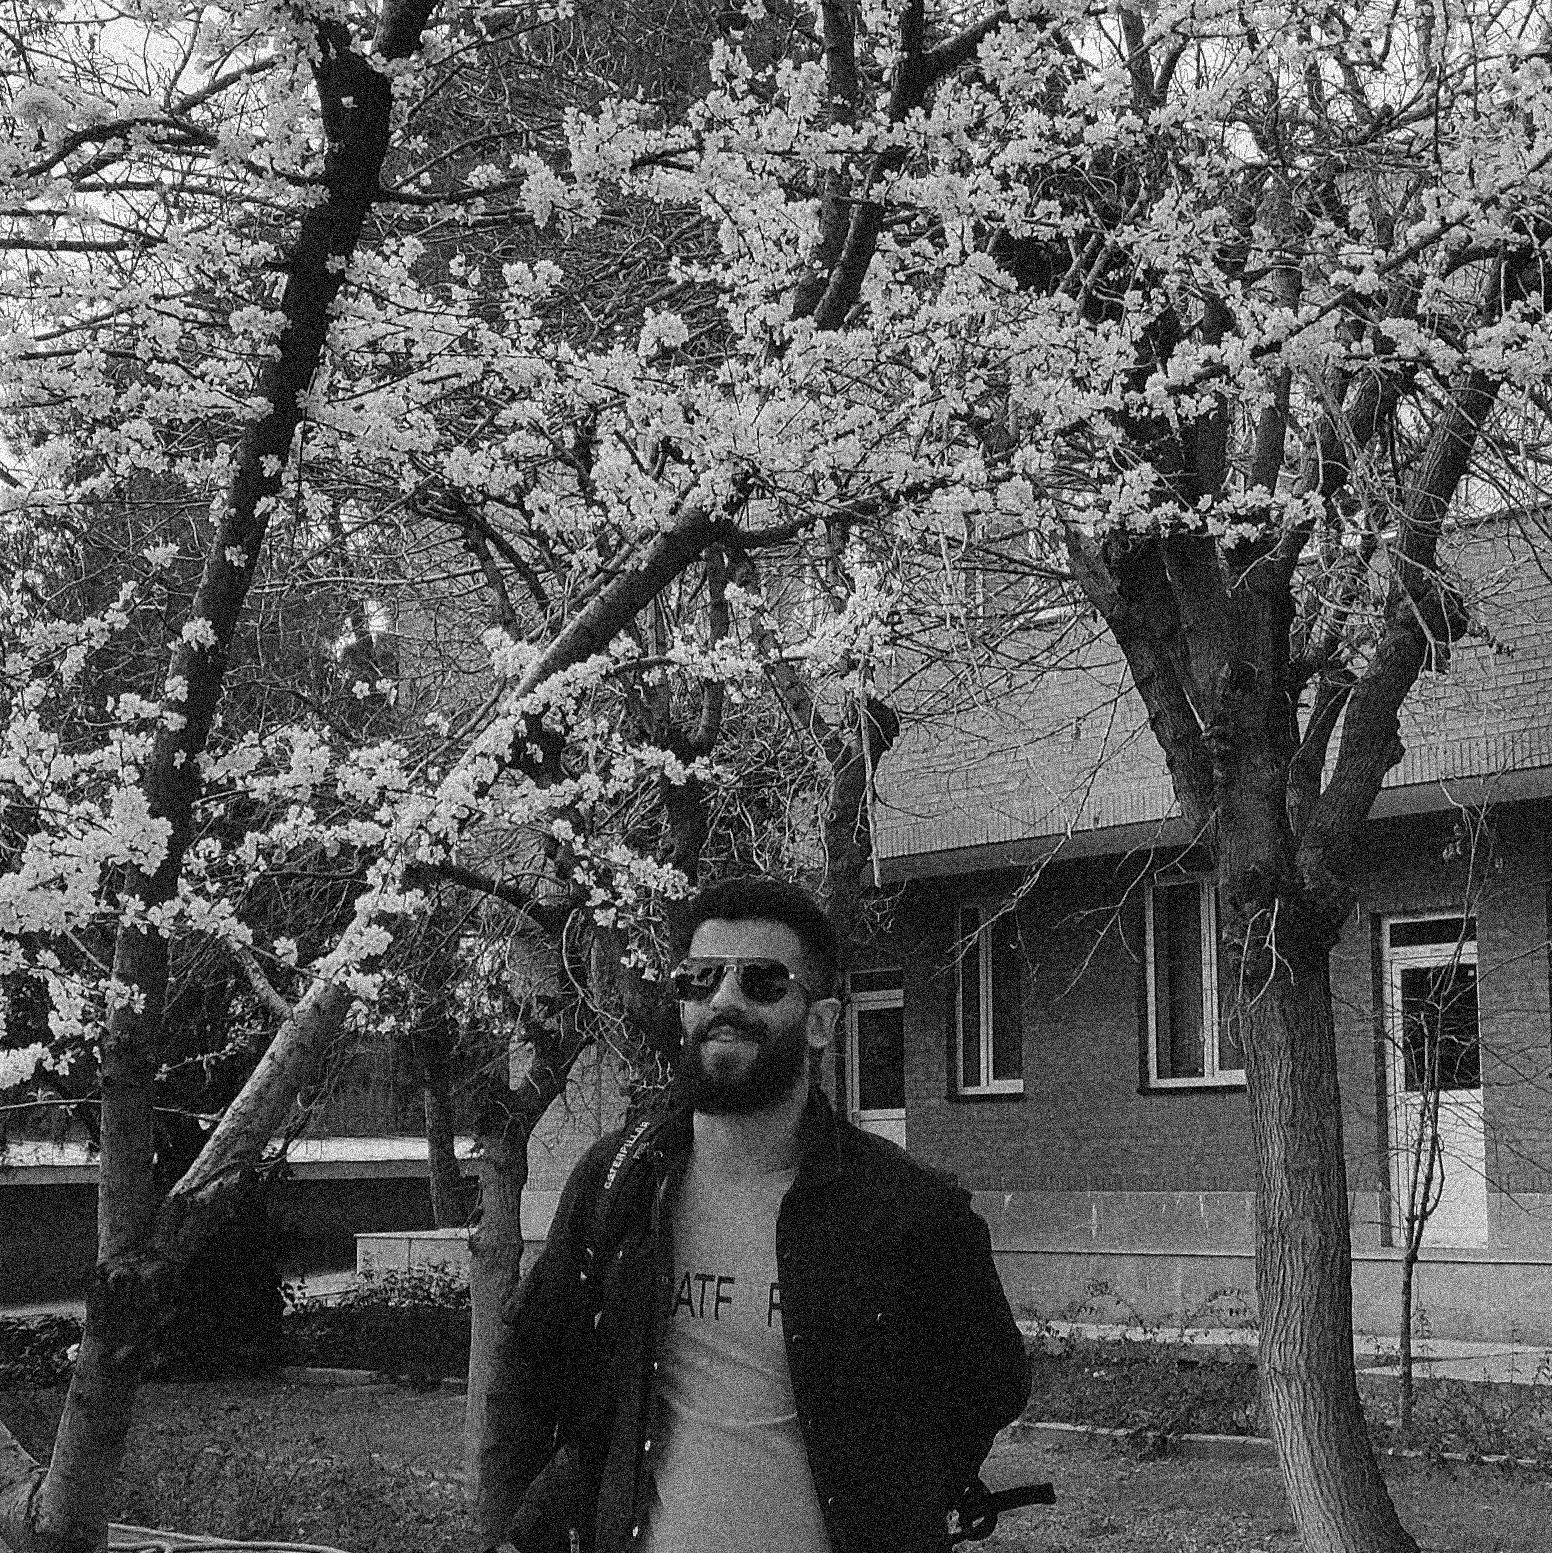
\includegraphics[width=0.65\linewidth]{images/noisyImage.jpg}
    \caption{ تصویر با نویز }
    \label{fig:h}
\end{figure}

\subsection{\lr{SNR(signal to noise ratio)}}
در این قسمت به محاسبه نسبت سینگال به نویزاضافه شده‌ می پردازیم. 
نسبت سیگنال به نویز، سطح توان سیگنال را با سطح توان نویز مقایسه می کند و معمولا بر حسب دسیبل بیان
می شود. هرچه مقدار نسبت سیگنال به نویز بیشتر باشد، برای یک سیستم مشخصه بهتری محسوب می شود؛
زیرا اطلاعات مفید بیشتری در قالب سیگنال، نسبت به اطلاعات ناخواسته یا نویز دریافت می شود.
\\
\grayBox{SNR}
:
میزان قدرت یک سیگنال نسبت به نویز پس‌زمینه آن می‌باشد.
که با با واحد 
\(db\)
اندازه‌گیری می‌شود.
\null \hfill $ SNR =  10 \cdot \log_{10} \dfrac{P_{signal}}{P_{noise}}$

این نسبت می‌تواند هر عددی باشد که اعداد بزرگتر از صفر نشان دهنده این است که سطح سیگنال اصلی بیشتر از سطح noise است 
و اعداد کوچکتر برعکس. 
در واقع هر چه این نسبت بزرگتر باشد کیفیت سیگنال بهتر است.
\BlankLine
توضیح مفصل تر:
\BlankLine
Signal-to-Noise Ratio
یک معیار است که در مورد نویز در عکس استفاده می‌شود. SNR نسبت سیگنال به نویز را نشان می‌دهد و از طریق اندازه‌گیری قدرت سیگنال نسبت به قدرت نویز، کیفیت سیگنال را ارزیابی می‌کند.

در مفهوم SNR، سیگنال نشان‌دهنده قسمت مورد نظر و معنادار تصویر است که می‌خواهیم دریافت کنیم. نویز، خراب‌کننده سیگنال است و می‌تواند از منابع مختلفی نظیر اندازه‌گیری ناقص، تداخل الکترومغناطیسی یا خطاهای فرآیند تولید تصویر، به وجود آید.

با اندازه‌گیری SNR، می‌توانیم نسبت قدرت سیگنال به قدرت نویز را محاسبه کنیم. این نسبت به صورت لگاریتمی بیان می‌شود و معمولاً به واحد دسی‌بل (dB) تبدیل می‌شود. بالاترین SNR ممکن، یعنی بی‌نویز بودن، معادل یک SNR بالغ بر بی‌نهایت است. در عمل، هدف ما افزایش SNR و کاهش نویز است تا سیگنال مورد نظر را بهتر و دقیق‌تر دریافت کنیم.

به عنوان مثال، در عکس‌برداری دیجیتال، SNR برای سنسور دوربین معیاری است که نشان می‌دهد درصد سیگنال واقعی تصویر (نسبت به سیگنال نویز) در میان اثرات نویزی ناشی از سنسور (نویز سیستمی) و شرایط نوری ضعیف (نویز محیطی) است. SNR بالا به معنای وجود کمترین نویز و سیگنال واضح و با کیفیت بالاست.
\subsection{بررسی کد}
\lr{\lstinputlisting{MatlabCode/snr.m}}

در این بخش اگر دو سیگنال را به صورت مستقبم به تابع از پیش تعریف‌شده 
\grayBox{snr}
میدادم به
\grayBox{syntax error}
برمی‌خوردم که می‌گفت باید ورودی های تابع 
\grayBox{snr}
باید 
\grayBox{double}
باشد در نتیجه هر دو سیگنال را به این نوع تبدیل کردم .
\\
علت اینکه دو نویز را از هم کم کرده‌ام این بود که باید نویز خالص را از این روش به دست می‌آوردم.

\grayLBox{signalNoiseRatio = 15.6827}


\section{گام هفتم}
در این گام سعی به گرفتن تبدیل فوریه از تصویر خاکستری شده و آن را طبق راهنمایی گفته شده رسم می‌کنیم.
همچنین برای حل این سوال با سرچ و خواندن مستندات سایت متلب و همچنین دانشی که از درس بینایی کامپیوتر کسب کرده ام استفاده کردم.
\\
\\
\\
\\
\subsection{بررسی کد}
\lr{\lstinputlisting{MatlabCode/step7.m}}

\begin{figure}[H]
    \centering
    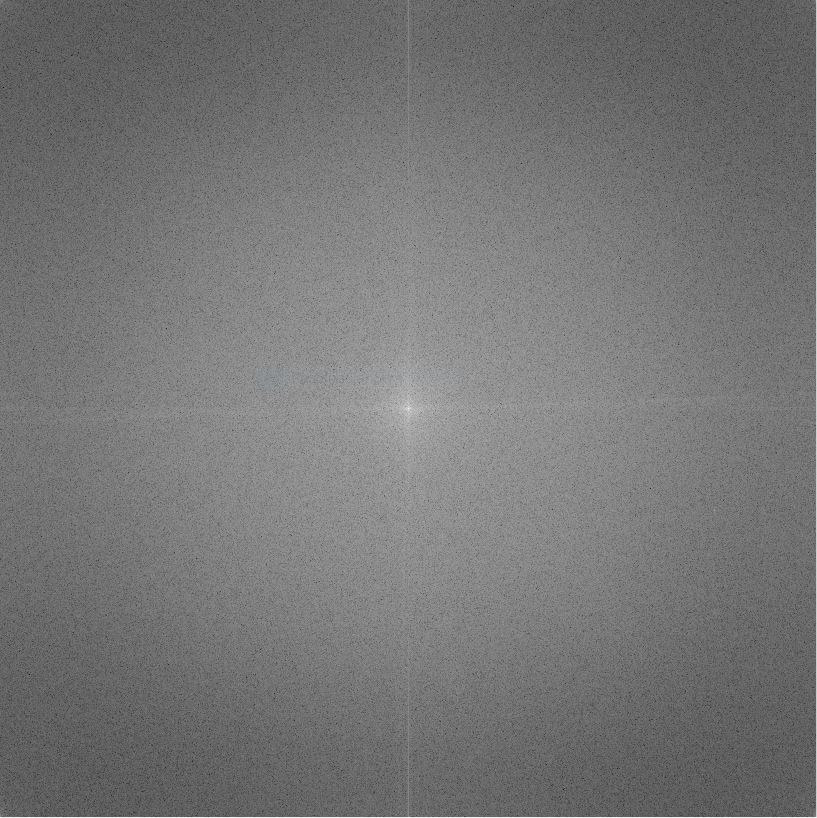
\includegraphics[width=0.65\linewidth]{images/fourierImage.jpg}
    \caption{ تصویر تبدیل فوریه گرفته شده }
    \label{fig:h}
\end{figure}

\subsection{تحلیل عکس بالا}
طی جست‌وجو های پی‌در‌پی نتایج دریافت‌شده از آنها را در قالب چند نکته اشاره می‌کنم:

\begin{itemize}
    \item هر پیکسل در عکس تبدیل فوریه نشان دهنده 
    یک موج سینوسی دو بعدی با فرکانس وابسته به فاصله از مرکز می‌باشد.
    \item نتیجه تصویر نشان می‌دهد که عکس حاوی تمامی فرکانس‌ها می‌باشد اما بزرگی آن هر چه از مرکز تصویر دورتر می‌شویم کمتر می‌شود و در نتیجه فرکانس بیشتر می‌شود.
    \item 
    فرکانس‌های کمتر حاوی اطلاعات بیشتری نسبت به فرکانس های بالاتر هستند.
    \item به طور معمول وسط عکس شامل فرکانس های
    بالاتر بوده ولی بعد از استفاده از دستود  fftshiftاوضاع تغییر کرد و وسط عکس نشانگر فرکانس های ⅼow
    شد.
\end{itemize}
\subsection{پاسخ به سوال‌ها}
\begin{enumerate}
    \item \textbf{مرکز تصویر چرا از همه نقاط دیگر نورانی تر است؟}
    به دلیل اینکه بخش زیادی از عکس فرکانس کمتری دارند و مرکز تصویر حاوی اطلاعات بیشتری است.
    به تعبیری دیگر بخش زیادی از تصویر اصلی ما داری تغییرات کم فرکانس هستند یعنی رنگ آنها به یک‌باره از سفید به سیاه تغییر نمی‌کند.
    همچنین نقطه مرکز دارای فرکانس صفر است و  از جمع مقادیر پیکسل ها (میانگین پیکسل ها) به دست می آیدو
    \item \textbf{چرا هر چه از مرکز دورتر می‌شویم نقاط کم نورتر می شوند؟}
    چون این نقاط فرکانس بیشتر را در بر می‌گیرند در واقع این نفاط نشان‌دهنده تغییر ناگهانی
    (فرکانس بالا)
    در عکس اصلی می‌باشند.
    \item \textbf{بالا و پایین‌ترین فرکانس در تصویر کدام نقاط است؟}
    مرکز دارای کمترین فرکانس و هرچه از مرکز دورتر می‌شویم فرکانس بیشتر می‌شود.
    بنابراین گوشه های تصویر دارای بیشترین فرکانس می‌باشند.
\end{enumerate}
\section{گام هشتم}
برای حل این سوال با توجه به صورت سوال ابتدا از تصویر تبدیل فوریه می گیریم.
سپس آن را شیفت می دهیم. بعد از آن فرکانس های پایین که در مرکز تصویر تبدیل فوریه قرار دارند را نگه می داریم و بقیه آن ها را دور میریزیم.
اصطلاحا آن را ماسک می کنیم. برای پیاده سازی نیز از سایت 
geeks for geeks
کمک گرفتم که در لینک های آخر گزارش قابل مشاده است.
پس از ماسک کردن فرکانس های بالا و نگه داشتن فرکانس های پایین از تصویر 
تبدیل فوریه معکوس میگیریم و قسمت حقیقی آن را نگه می داریم.
در تصویر حاصل نویز رفع شده است ولی کمی کیفیت تصویر کاهش یافته است و لبه های آن از بین رفته اند .
\BlankLine
همچنین روش دوم یا جایگزینی هم وجود دارد که به شرح زیر است.
با کمک گرفتن از مستند اصلی سایت متلب از روش 
\grayBox{\(median\)}
(فیلتر میانه)
استفاده می‌کنیم که این متد با کمک
\(3-by-3 neighborhood\)
پیاده‌سازی شده‌است.
فیلتر میانه که یک فیلتر مرتبه ای است برای نویز نمک و فلفل بسیار مناسب است.
همچنین این فیلتر برای حذف نویز هایی که در تصویر ما وجود دارد بسیار مناسب است.
\subsection{بررسی کد}
\lr{\lstinputlisting{MatlabCode/step8.m}}

\begin{figure}[H]
    \centering
    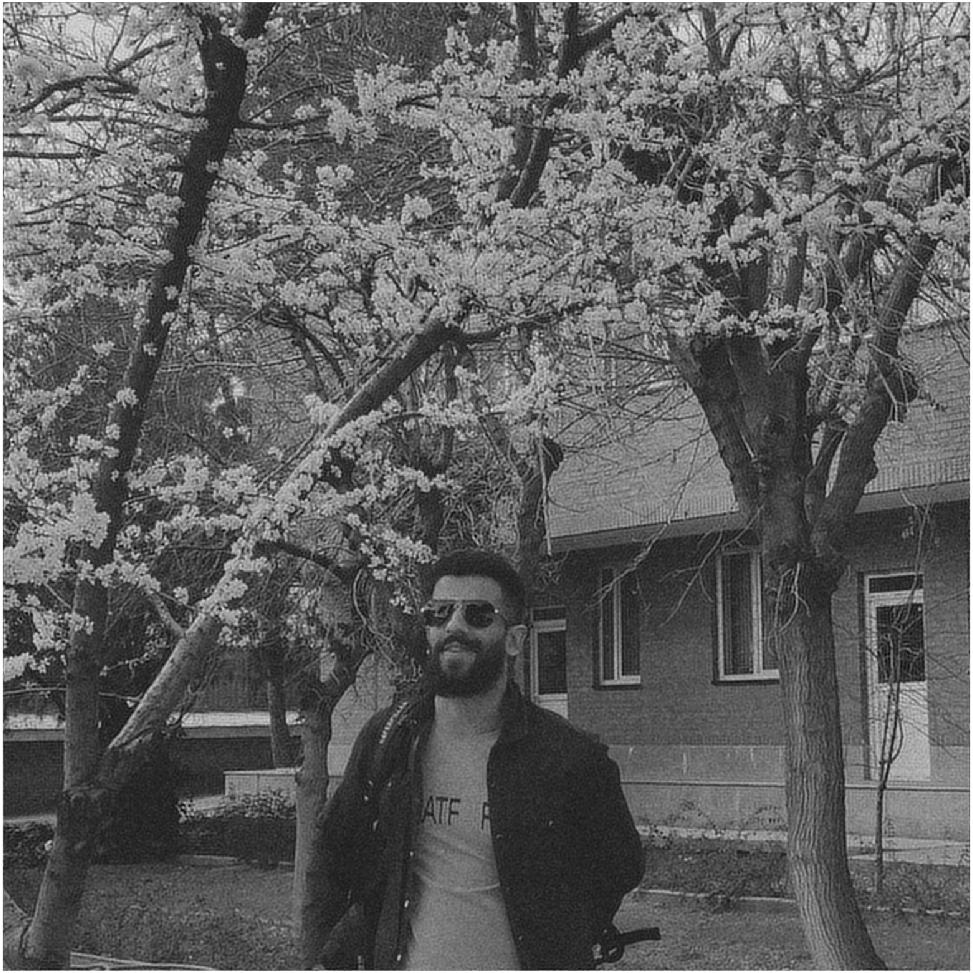
\includegraphics[width=0.65\linewidth]{images/removedNoise.jpg}
    \caption{ تصویر با نویز رفع‌شده }
    \label{fig:h}
\end{figure}

\subsection{عملکرد رفع نویز }
با توجه به راهنمایی گفته‌شده و تابع ازپیش‌تعریف‌شده 
\grayBox{\(PSNR\)}
به بررسی این تابع می‌پردازیم
.
هرچه مقدار خروجی این تابع بیشتر باشد ما بهتر عمل کرده‌ایم
\subsubsection{PSNR range}
\begin{itemize}
    \item برای تصویر ها و ویدئو های فشرده شده بین 
    ۳۰ تا ۵۰ دسی‌بل می‌باشد
    که ۸ بیتی است.
    \item برای ۱۲ بیتی خروجی از ۶۰ به بالا خوب است
    \item مقدارهای قابل‌قبول برای انتقال‌های بی‌سیم بین ۲۰ تا ۲۵ می‌باشد.
\end{itemize}
\lr{\lstinputlisting{MatlabCode/peakSNR.m}}

\grayLBox{The Peak-SNR value is 20.4128}

\subsubsection{توضیح تکمیلی PSNR}
PSNR یک معیار است که برای ارزیابی کیفیت تصاویر مورد استفاده قرار می‌گیرد. این معیار با توجه به نسبت بیشینه سیگنال به نویز، ارزیابی کیفیت تصویر را انجام می‌دهد.

PSNR بر اساس مقایسه سیگنال واقعی (تصویر اصلی یا مرجع) با تصویر بازسازی شده (تصویر پردازش شده) اندازه‌گیری می‌شود. برای محاسبه PSNR، ابتدا نسخه بازسازی شده تصویر باید با تصویر اصلی مقایسه شود و سیگنال خطا (تفاوت بین دو تصویر) یا نویز محاسبه می‌شود. سپس با استفاده از فرمول مربوطه، PSNR بر اساس مقدار بیشینه ممکن برای سیگنال واقعی (با توجه به بیت‌های نمایش) و مقدار میانگین مربعات خطا (MSE) محاسبه می‌شود.

به طور کلی، مقادیر PSNR بیشتر نشان دهنده کیفیت بالاتر تصویر هستند. افزایش مقدار PSNR به معنای کاهش نویز و افزایش تطابق تصویر با تصویر اصلی است. با این حال، باید توجه داشت که PSNR تنها یکی از معیارهای موجود برای ارزیابی کیفیت تصویر است و ممکن است به عنوان یک معیار کمی، به برخی جنبه‌های کیفیت تصویر، مانند واقعیت رنگ یا وضوح جزئیات، توجه نکند.

بنابراین، PSNR می‌تواند به عنوان یک معیار کمکی برای ارزیابی کیفیت تصاویر مورد استفاده قرار گیرد، اما برای ارزیابی کامل و جامع تصاویر، معیارهای دیگری مانند 
\grayBox{\(SSIM (Structural Similarity Index) \)}
و
\grayBox{\(VIF (Visual Information Fidelity)\)}
نیز ممکن است مورد استفاده قرار بگیرند.